\documentclass[12pt]{exam}

% essential packages
\usepackage{fullpage} % margin formatting
\usepackage{enumitem} % configure enumerate and itemize
\usepackage{amsmath, amsfonts, amssymb, mathtools} % math symbols
\usepackage{xcolor, colortbl} % colors, including in tables
\usepackage{makecell} % thicker \Xhline in table
\usepackage{graphicx} % images, resizing
\usepackage{tikz} % drawing graphs
\usetikzlibrary{positioning}

% sometimes needed packages
\usepackage{hyperref} % hyperlinks
% \hypersetup{colorlinks=true, urlcolor=blue}
% \usepackage{logicproof} % natural deduction
% \usepackage{tikz} % drawing graphs
% \usetikzlibrary{positioning}
% \usepackage{multicol}
% \usepackage{algpseudocode} % pseudocode

% paragraph formatting
\setlength{\parskip}{6pt}
\setlength{\parindent}{0cm}

% newline after Solution:
\renewcommand{\solutiontitle}{\noindent\textbf{Solution:}\par\noindent}

% less space before itemize/enumerate
\setlist{topsep=0pt}

% creates \filcl to grey out cells for groupwork grading
\newcommand{\filcl}{\cellcolor{gray!25}}

% creates \probnum to get the problem number
\newcounter{probnumcount}
\setcounter{probnumcount}{1}
\newcommand{\probnum}{\arabic{probnumcount}. \addtocounter{probnumcount}{1}}

% use roman numerals by default
\setlist[enumerate]{label={(\roman*)}}

% creates custom list environments for grading guidelines, question parts
\newlist{guidelines}{itemize}{1}
\setlist[guidelines]{label={}, left=0pt .. \parindent, nosep}
\newlist{gwguidelines}{enumerate}{1}
\setlist[gwguidelines]{label={(\roman*)}, nosep}
\newlist{qparts}{enumerate}{2}
\setlist[qparts]{label={(\alph*)}}
\newlist{qsubparts}{enumerate}{2}
\setlist[qsubparts]{label={(\roman*)}}
\newlist{stmts}{enumerate}{1}
\setlist[stmts]{label={(\roman*)}, nosep}
\newlist{pflist}{itemize}{4}
\setlist[pflist]{label={$\bullet$}, nosep}
\newlist{enumpflist}{enumerate}{4}
\setlist[enumpflist]{label={(\arabic*)}, nosep}

\printanswers

\begin{document}
%%%%%%%%%%%%%%% TITLE PAGE %%%%%%%%%%%%%%%
\title{EECS 203: Discrete Mathematics\\
  Fall 2023\\
  Homework 9}
\date{}
\author{}
\maketitle
\vspace{-50pt}
\begin{center}
  \huge Due \textbf{Thursday, November 16}, 10:00 pm\\
\Large No late homework accepted past midnight.\\
\vspace{10pt}
\large Number of Problems: $9+2$
\hspace{3cm}
Total Points: $100+30$
\end{center}
\vspace{25pt}
\begin{itemize}
    \item \textbf{Match your pages!} Your submission time is when you upload the file, so the time you take to match pages doesn't count against you.
    \item Submit this assignment (and any regrade requests later) on Gradescope. 
    \item Justify your answers and show your work (unless a question says otherwise).
    \item By submitting this homework, you agree that you are in compliance with the Engineering Honor Code and the Course Policies for 203, and that you are submitting your own work.
    \item Check the syllabus for full details.
\end{itemize}
\newpage
%%%%%%%%%%%%%%% TITLE PAGE %%%%%%%%%%%%%%% 

\section*{Individual Portion}

\subsection*{\probnum Shortest Paths [12 points]}
Provide the shortest path distances between the following point pairings in their respective graphs.  Justify your answer by providing a shortest path, or by stating that there is no such path.
\begin{qparts}
    \item 
    
    \begin{qsubparts}
        \item $(x, p)$
        \item $(c, o)$\\
        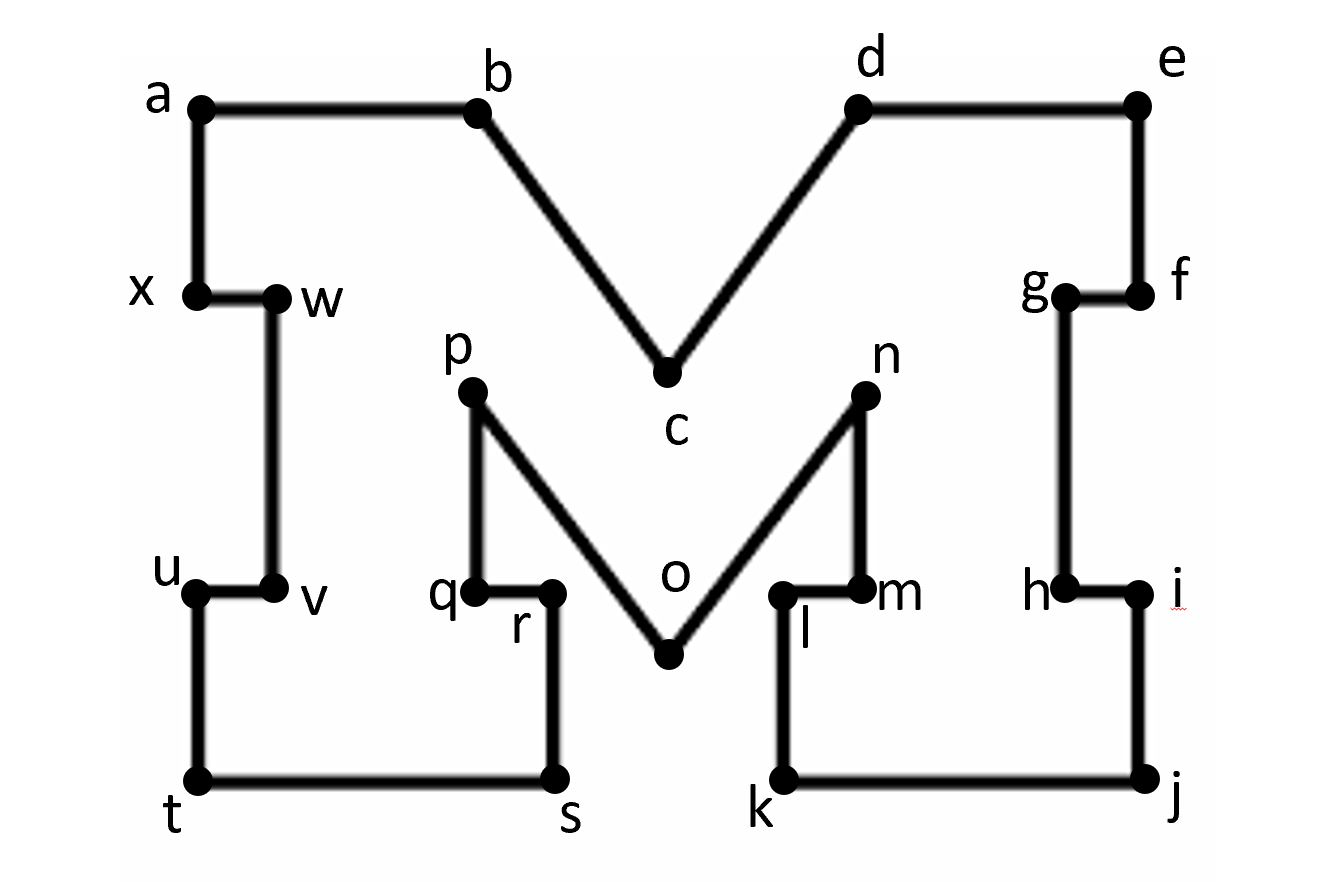
\includegraphics[width=0.5\textwidth]{pointy_m.JPG}
    \end{qsubparts}
    \item
    \begin{qsubparts}
        \item $(a, z)$
        \item $(b, j)$\\
        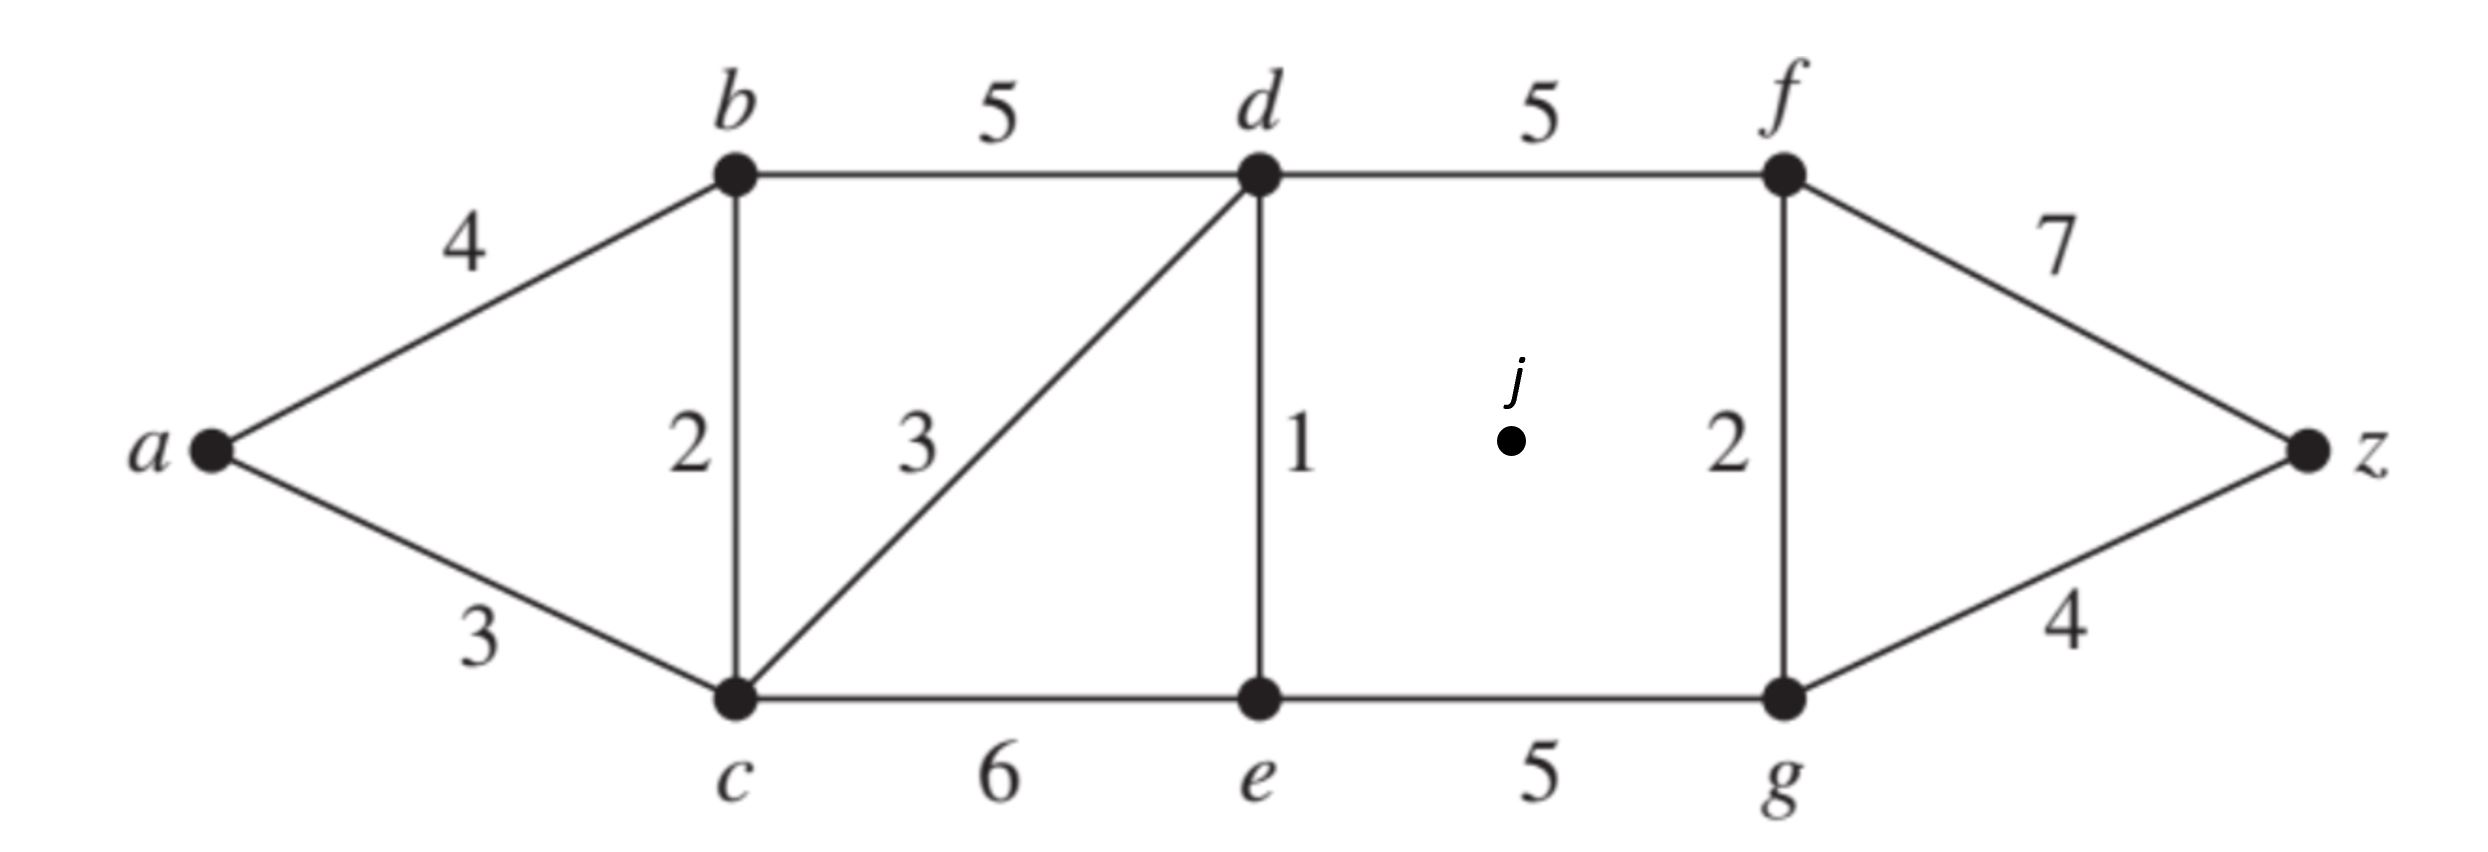
\includegraphics[width=0.7\textwidth]{weighted_graph.JPG}
    \end{qsubparts}
    \newpage
    \item 
        \begin{qsubparts}
        \item $(a, g)$
        \item $(i, b)$\\
        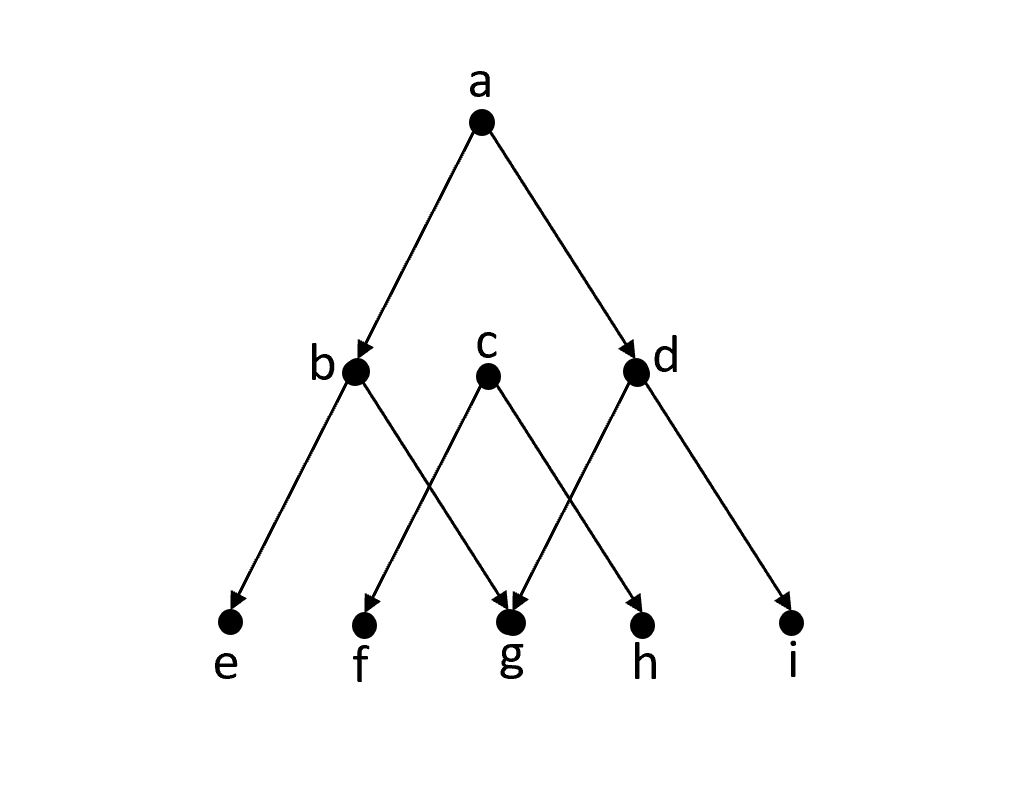
\includegraphics[width=0.4\textwidth]{tree.JPG}
    \end{qsubparts}
\end{qparts}


\begin{solution}
    \begin{qparts}
        \item 
        ~\\ 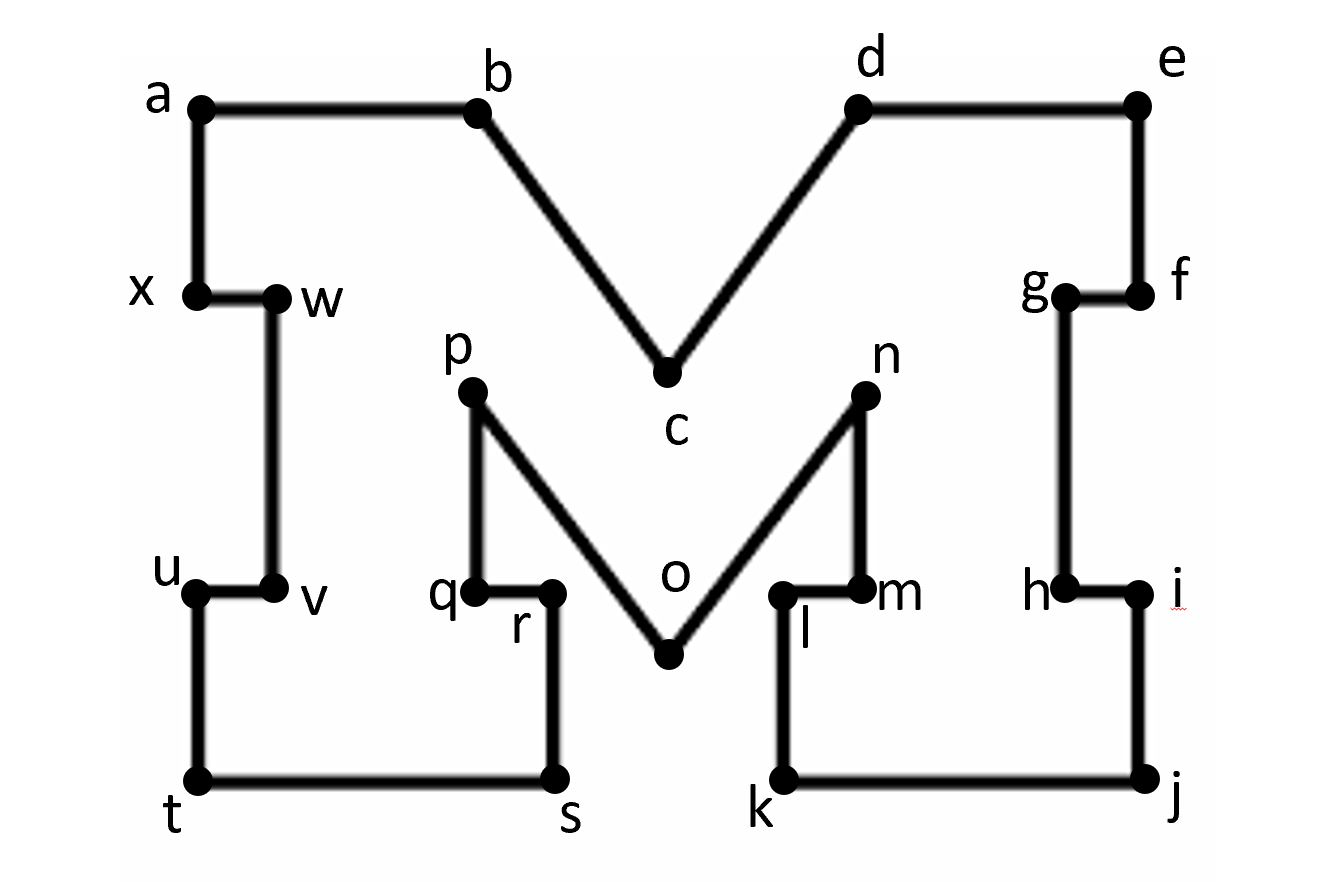
\includegraphics[width=0.5\textwidth]{pointy_m.JPG}
        ~\\~\\~\\~\\~\\~\\~\\
        \item
        ~\\ 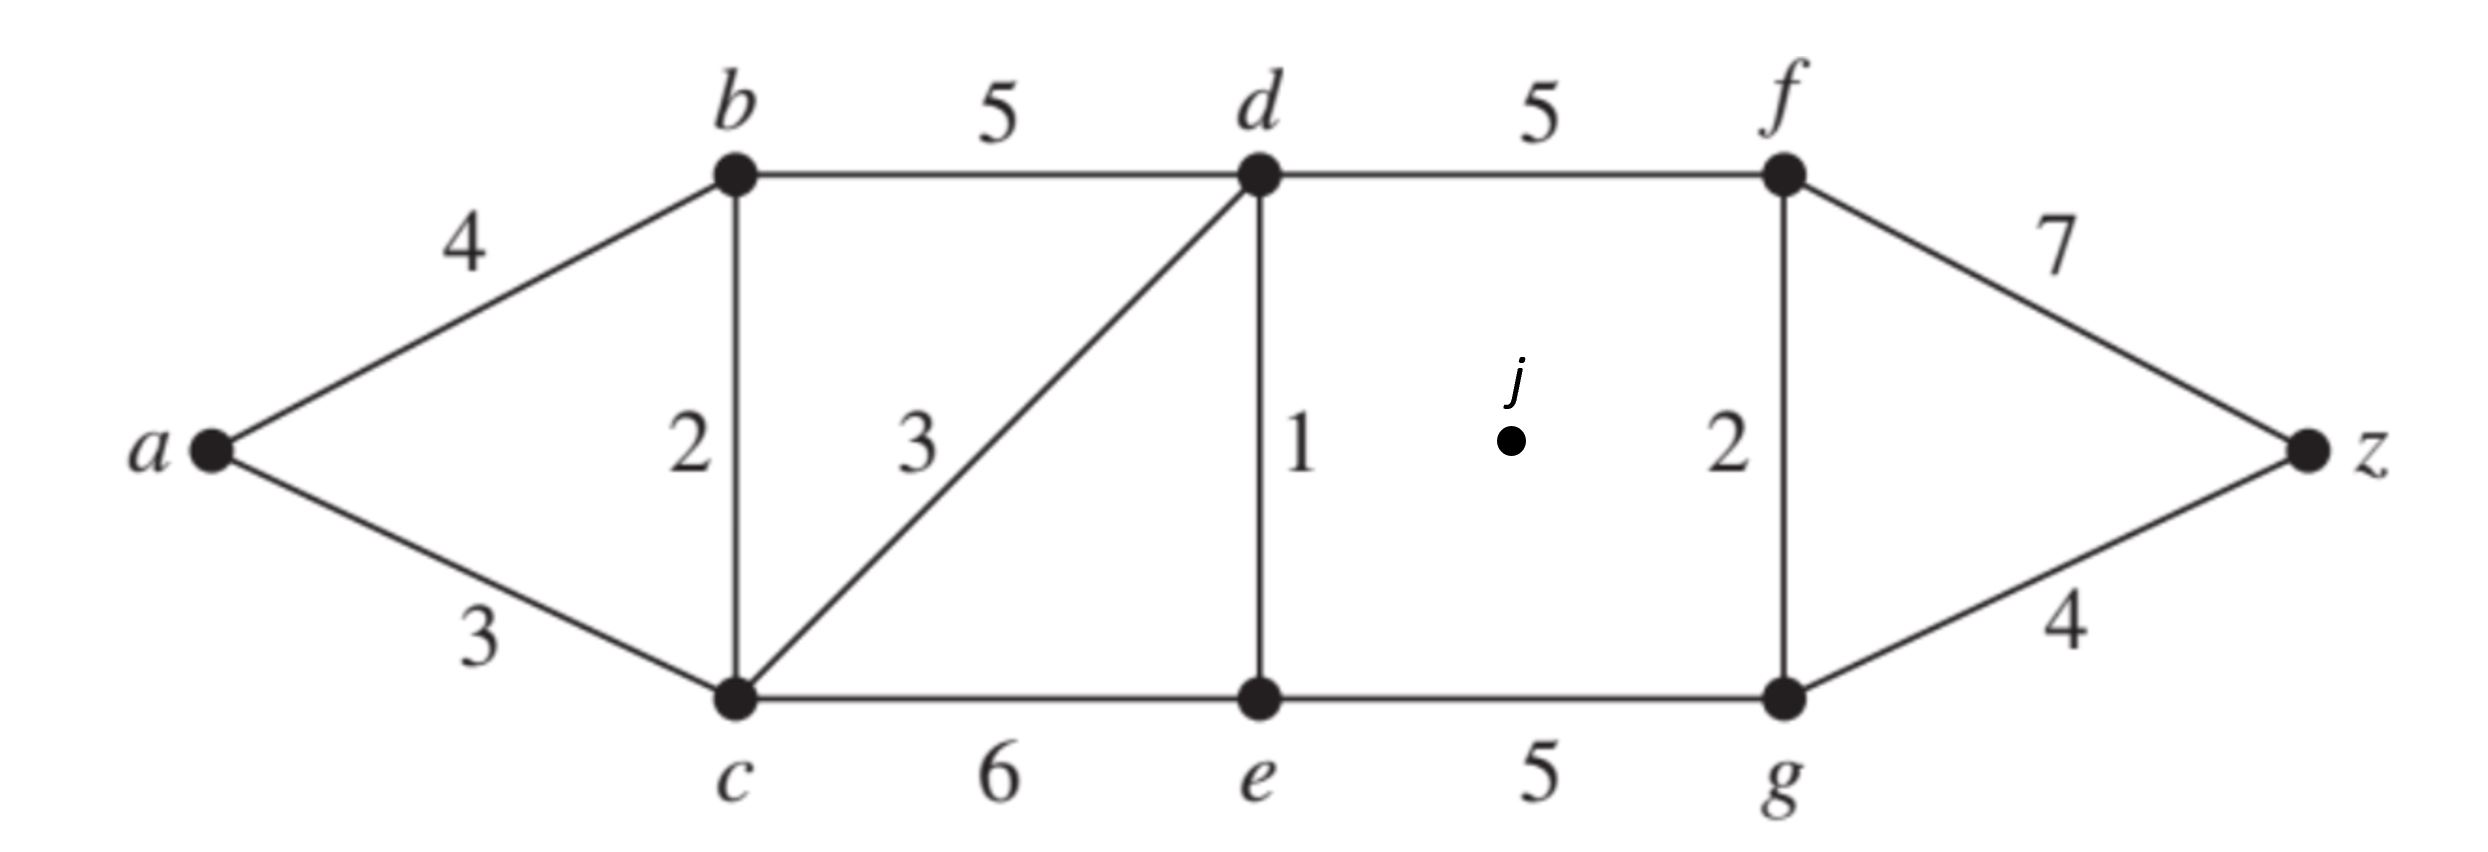
\includegraphics[width=0.7\textwidth]{weighted_graph.JPG}
        ~\\~\\~\\~\\~\\~\\~\\
        \item 
        ~\\ 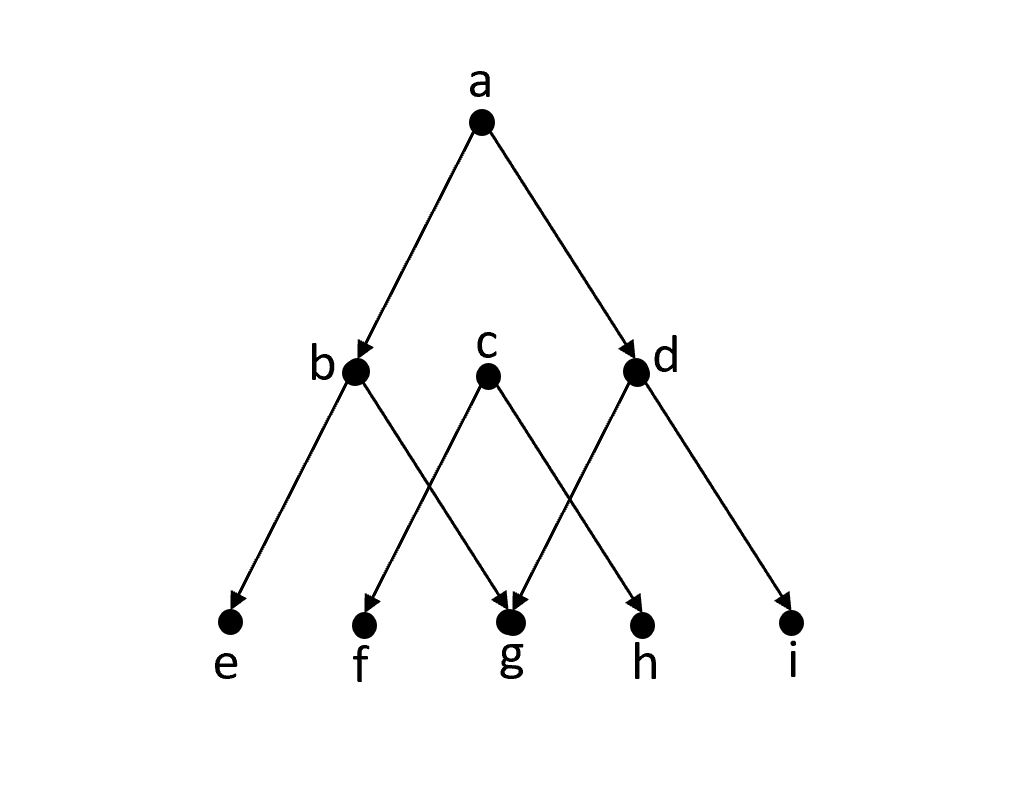
\includegraphics[width=0.4\textwidth]{tree.JPG}
        ~\\~\\~\\~\\~\\~\\~\\
    \end{qparts}
\end{solution}

\subsection*{\probnum Alexander Hamiltonian [12 points]}
For each of the following parts, state whether a graph with $n\geq{3}$ vertices and the given properties \textbf{always}, \textbf{sometimes}, or \textbf{never} contains a Hamiltonian cycle. Justify your response for each part. 
\begin{qparts}
    \item The complete graph $K_n$. 
    \item A tree.
    \item A bipartite graph. 
    \item A graph that contains a vertex $v$ where $\text{deg}(v) = 1$. 
\end{qparts}

\begin{solution}
    \begin{qparts}
        \item
        ~\\~\\~\\~\\~\\~\\~\\~\\~\\~\\~\\~\\~\\~\\
        \item
        ~\\~\\~\\~\\~\\~\\~\\~\\~\\~\\~\\~\\~\\~\\
        \item
        ~\\~\\~\\~\\~\\~\\~\\~\\~\\~\\~\\~\\~\\~\\
        \item
        ~\\~\\~\\~\\~\\~\\~\\~\\~\\~\\~\\~\\~\\~\\
    \end{qparts}
\end{solution}

\subsection*{\probnum Bipartite? [12 points]}
For each of the following parts, determine if the graph is bipartite and justify your answer.
\begin{qparts}
    \item The cycle $C_5$
    \item The hypercube $Q_2$
    \item The complete graph $K_5$
    \item ~\\
    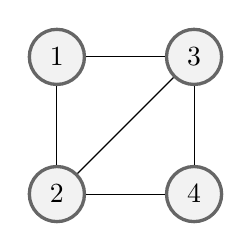
\begin{tikzpicture}[
    roundnode/.style={circle, draw=black!60, fill=gray!10, very thick, minimum size=7mm},
    ]

    \node[roundnode] (1) {1};
    \node[roundnode] (2) [below=of 1] {2};
    \node[roundnode] (3) [right=of 1] {3};
    \node[roundnode] (4) [below=of 3] {4};
    
    \draw[-] (3)--(4);
    \draw[-] (1)--(3);
    \draw[-] (2)--(3);
    \draw[-] (4)--(2);
    \draw[-] (2)--(1);
    \end{tikzpicture}
\end{qparts}
\begin{solution}   
    \begin{qparts}
        \item 
        ~\\~\\~\\~\\~\\~\\~\\~\\
        \item 
        ~\\~\\~\\~\\~\\~\\~\\~\\
        \item 
        ~\\~\\~\\~\\~\\~\\~\\~\\
        \item
        ~\\~\\~\\~\\~\\~\\~\\~\\~\\~\\~\\~\\~\\
    \end{qparts}
\end{solution}


\subsection*{\probnum Melman the Graph [12 points]}
In a simple, undirected graph with $5$ vertices, what are all possible values for the number of vertices with odd degree? Justify your answer.

For each possible value $k$, construct a graph with 5 vertices that has $k$ vertices of odd degree.

\begin{solution}
    ~\\~\\~\\~\\~\\~\\~\\~\\~\\~\\~\\~\\~\\~\\
\end{solution}

\subsection*{\probnum Keeping things Merry! [12 points]}

Mary has three dogs, Sarge, Duke, and Brady. However, when left alone, Duke will pick a fight with either of the other two dogs. Mary wants to walk all 3 dogs from her house across the road to the dog park, can only walk 1 dog at a time, and wants to avoid a fight between any of the dogs. She can make multiple trips across the road, and can leave some of her dogs on one side of the road when walking another across.

\begin{qparts}
    \item Draw a graph where the nodes are the legal configurations of the puzzle and the edges represent possible transitions from one state to another. Each node should contain M, S, D, B, and $||$ representing Mary, Sarge, Duke, Brady, and the road. For instance SB$||$MD would represent the Sarge and Brady being the the left side of the road at home with Mary and Duke on the other side at the park. Start with MSDB$||$ as your initial state.

    \item Identify the nodes that represent the start and end configurations of the puzzle. Is the puzzle solvable? Explain in terms of your graph.
\end{qparts}

\begin{solution}
    \begin{qparts}
        \item 
        ~\\~\\~\\~\\~\\~\\~\\~\\~\\~\\~\\~\\~\\~\\
        \item
        ~\\~\\~\\~\\~\\~\\~\\~\\~\\~\\~\\~\\~\\~\\
    \end{qparts}

\end{solution}


\subsection*{\probnum It's Iso-Morphin' Time [12 points]}
Determine whether or not each of the following pairs of graphs are isomorphic. If yes, provide an isomorphism. If not, explain why.
\begin{qparts}
   \item ~\\ 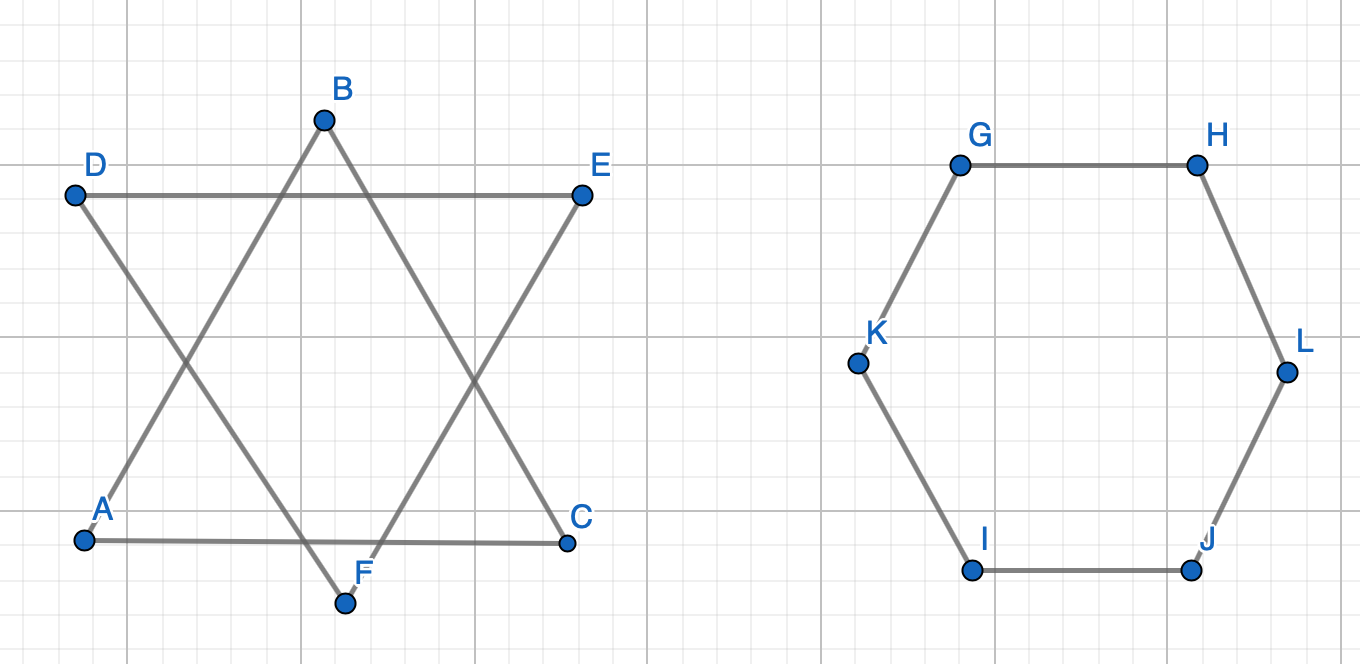
\includegraphics[width=30em]{isomorphism 1.png}
    \item ~\\ 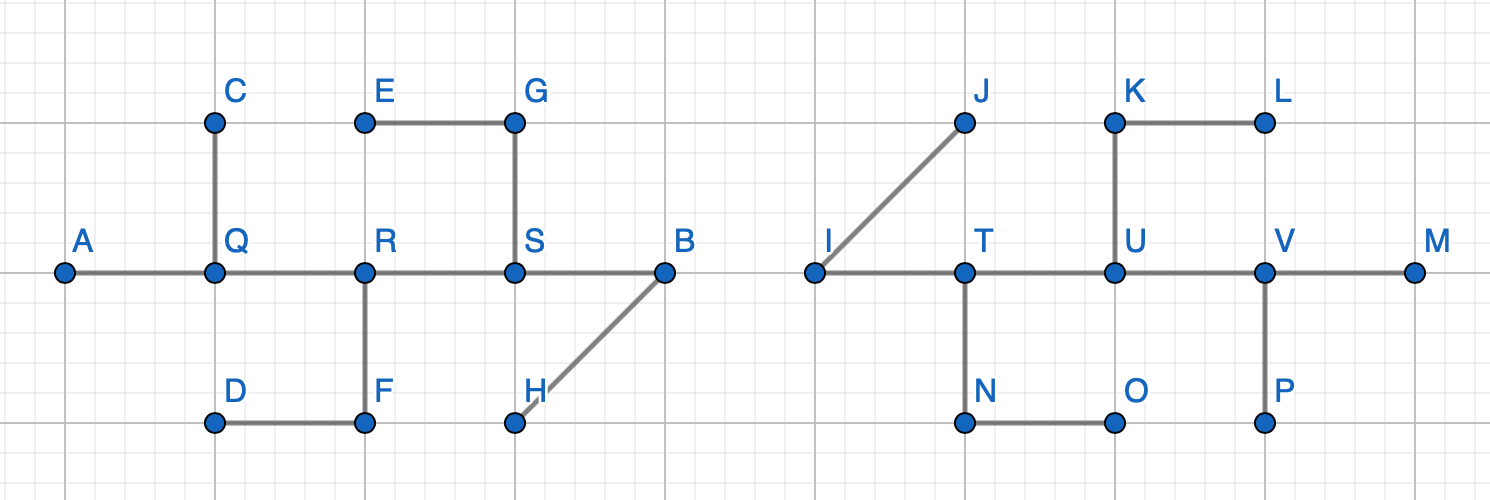
\includegraphics[width=30em]{isomorphism 4.png}
    \item ~\\ 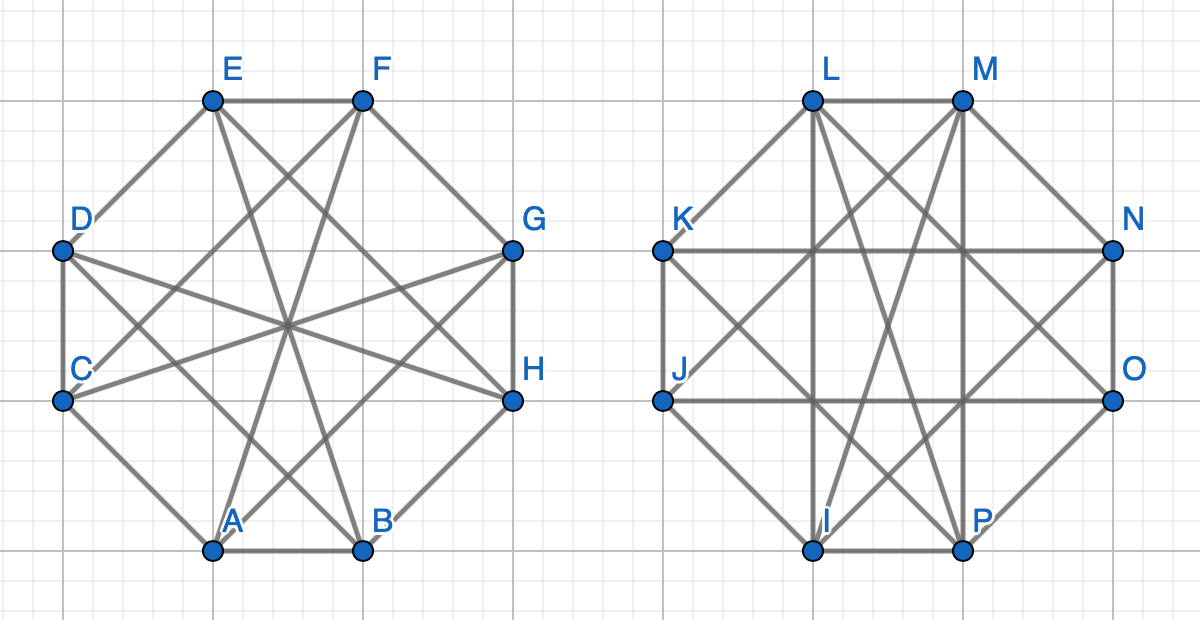
\includegraphics[width=30em]{isomorphism 5.png}
\end{qparts}

\begin{solution} 
    \begin{qparts}
        \item ~\\ 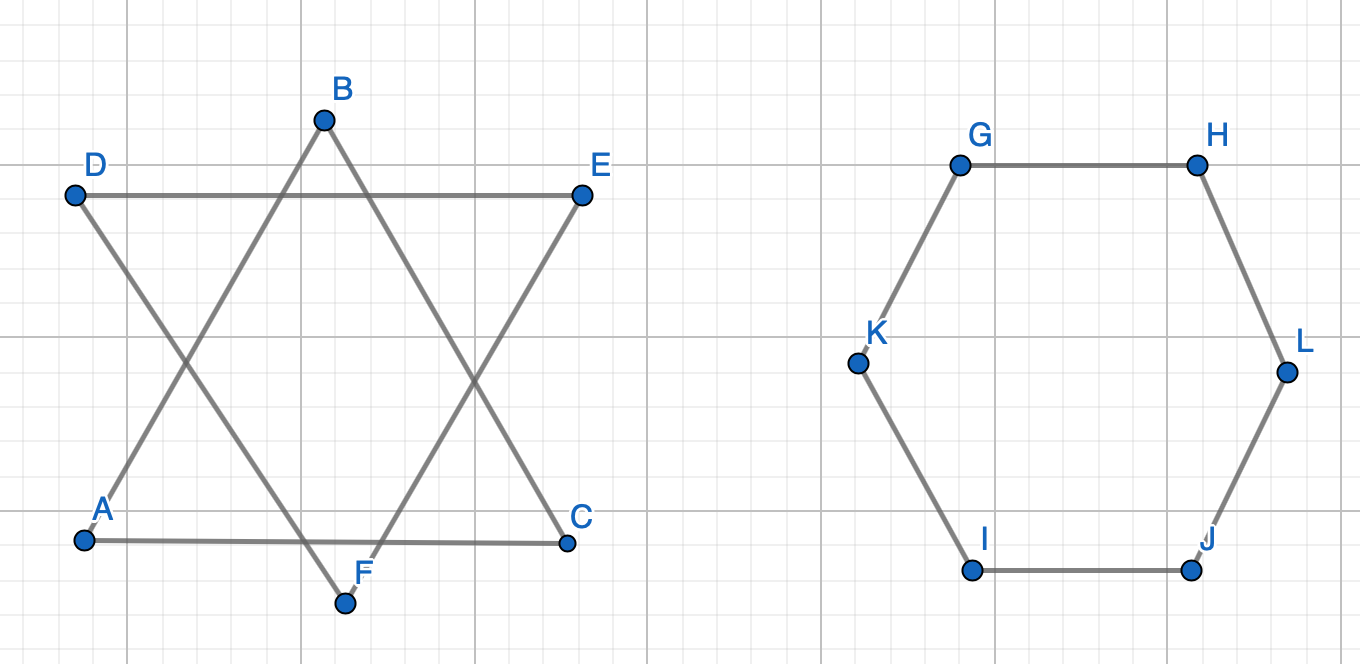
\includegraphics[width=30em]{isomorphism 1.png}
        ~\\~\\~\\~\\~\\~\\~\\~\\~\\~\\~\\~\\~\\~\\
        \item ~\\ 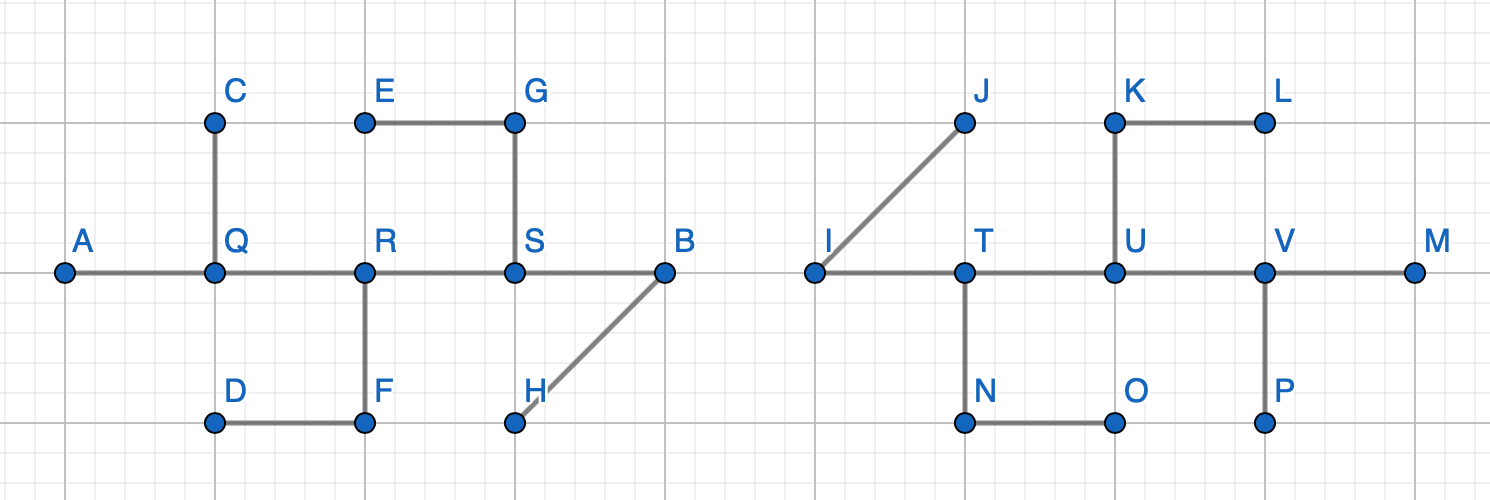
\includegraphics[width=30em]{isomorphism 4.png}
        ~\\~\\~\\~\\~\\~\\~\\~\\~\\~\\~\\~\\~\\~\\
        \item ~\\ 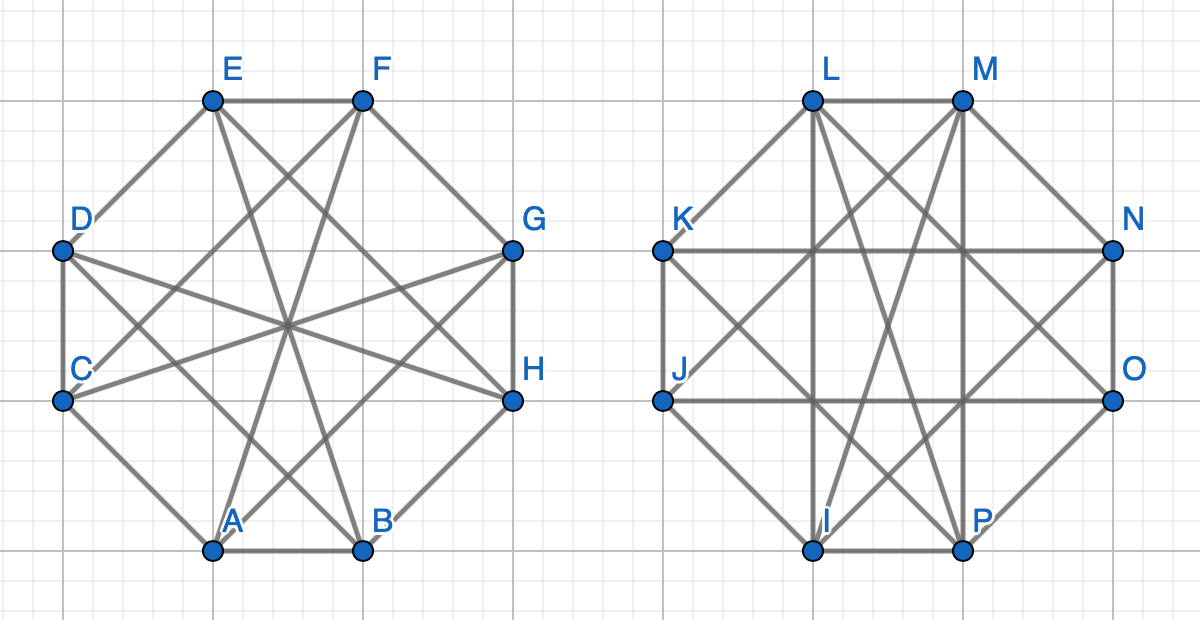
\includegraphics[width=30em]{isomorphism 5.png}
        ~\\~\\~\\~\\~\\~\\~\\~\\~\\~\\~\\~\\~\\~\\~\\~\\~\\~\\~\\
    \end{qparts}
\end{solution}


\subsection*{\probnum Reduce, Reuse, Recycle [12 points]}
For which values of $n\ge 4$ do these graphs have an Euler cycle?
\begin{qparts}
    \item The complete graph $K_n$
    \item The cycle $C_n$
    \item The wheel $W_n$
    \item The hypercube $Q_n$
\end{qparts}
\begin{solution}
    \begin{qparts}
        \item ~\\~\\~\\~\\~\\~\\~\\~\\~\\~\\~\\~\\~\\
        \item ~\\~\\~\\~\\~\\~\\~\\~\\~\\~\\~\\~\\~\\
        \item ~\\~\\~\\~\\~\\~\\~\\~\\~\\~\\~\\~\\~\\
        \item ~\\~\\~\\~\\~\\~\\~\\~\\~\\~\\~\\~\\~\\
    \end{qparts}
\end{solution}


\subsection*{\probnum Counting [8 points]}
How many positive integers less than 1000
\begin{qparts}
    \item are divisible by 7 but not by 11? 
    \item have distinct digits? 
    \item have distinct digits and are even?
\end{qparts}

You do \textbf{not} need to simplify your answer.

\begin{solution}
    \begin{qparts}
        \item ~\\~\\~\\~\\~\\~\\~\\~\\~\\
        \item ~\\~\\~\\~\\~\\~\\~\\~\\~\\
        \item ~\\~\\~\\~\\~\\~\\~\\~\\~\\
    \end{qparts}
\end{solution}


\subsection*{\probnum (Not So) Round and Round [8 points]}
Suppose we have a square-shaped table which seats 3 people on each side. How many ways are there to seat 12 people at the table, where seatings are considered the same if everyone is in the same group of 3 on a side?

\begin{solution}
    ~\\~\\~\\~\\~\\~\\~\\~\\~\\~\\~\\~\\~\\
\end{solution}

\pagebreak
\setcounter{probnumcount}{1}
\section*{Groupwork}
\subsection*{\probnum Grade Groupwork 8}
Using the solutions and Grading Guidelines, grade your Groupwork 8:
\begin{itemize}
    \item Mark up your past groupwork and submit it with this one.
    \item Write whether your submission achieved each rubric item. If it didn't achieve one, say why not.
    \item Use the table below to calculate scores.
    \item For extra credit, write positive comment(s) about your work.
    \item You don't have to redo problems correctly, but it is recommended!
    \item What if my group changed? \begin{itemize}
        \item If your current group submitted the same groupwork last time, grade it together.
        \item  If not, grade your version, which means submitting this groupwork assignment separately. You may discuss grading together.
    \end{itemize}
\end{itemize}

\begin{center}
\resizebox{\textwidth}{!}{\begin{tabular}{| c | c | c | c | c | c | c | c | c | c | c | c | c |}
\hline
 & (i) & (ii) & (iii) & (iv) & (v) & (vi) & (vii) & (viii) & (ix) & (x) & (xi) & Total:\\
\hline
Problem 2 & & & & & &\filcl &\filcl &\filcl &\filcl & \filcl& \filcl& \hspace{1cm}/12\\
\hline 
Problem 3 & & & & & & & &\filcl &\filcl & \filcl& \filcl& \hspace{1cm}/30\\
\Xhline{1.25pt}
Total: &\filcl &\filcl &\filcl &\filcl &\filcl &\filcl &\filcl &\filcl & \filcl& \filcl& \filcl&\hspace{1cm}/42\\
\hline
\end{tabular}}
\end{center}

\subsection*{Previous Groupwork 8(1): Divisibility by Seven [12 points]}

In this question we will show that, given a 7-digit number, where all digits except perhaps the last are non-zero, you can cross out some digits at the beginning and at the end such that the remaining number consists of at least one digit and is divisible by 7. You are allowed to cross off zero digits.

For example, if we take the number 1234589, then we can cross out 1 at the beginning and 89 at the end to get the number $2345 = 7 \cdot 335$.

We will label the digits of an arbitrary 7-digit number as $$x_6 x_5 x_4 x_3 x_2 x_1 x_0.$$
\begin{qparts}
    \item Prove that there exists some $i < 7$ such that either $x_i x_{i-1} \dots x_0$ is divisible by 7,
    or, if it isn't, then there exists some $j < i$ such that $x_j x_{j-1} \dots x_0$ is congruent to it
    modulo 7.
    \item Use part (a) to prove that if there does not exist some $i < 7$ such that $x_i x_{i-1} \dots x_0$ is divisible by 7, then there exists $7 > i > j \geq 0$ so that $$\underbrace{x_ix_{i-1}\dots x_{j+1} 0 \dots 0}_{i + 1 \text{ digits total}}$$ is divisible by 7.
    \item Prove the full claim. That is, show that, given a 7-digit number, where all digits except perhaps the last are non-zero, you can cross out some digits at the beginning and at the end such that the remaining number consists of at least one digit and is divisible by 7.
\end{qparts}
\begin{solution} 
    \begin{qparts}
        \item
        There are 7 numbers: $x_6 x_5 x_4 x_3 x_2 x_1 x_0$, $x_5 x_4 x_3 x_2 x_1 x_0$, $\cdots$, $x_0$.\\
        Use them as Pigeons.\\
        The remainer of any number mod 7, if the number cannot be divided by 7, has 6 circumstances: 1,2,3,4,5,6.\\
        Use them as Holes.\\
        Assume that all these 7 numbers is not divisible by 7, then there are 7 Pigeons in 6 holes, which means that there are at least 2 Pigeons in one whole.\\
        This means that $i < 7$ and $j < i$ such that $ = x_i x_{i-1} \dots x_0$ and $x_j x_{j-1} \dots x_0$ have the same remainer when divided by 7.\\
        Mark the two numbers as $a $ and $b$.\\
        Then $b \equiv a \pmod{7}$.\\
        $(b-a) \equiv 0 \pmod{7}$.\\
        Then we have proved the statement: There exists some $i < 7$ such that either $x_i x_{i-1} \dots x_0$ is divisible by 7,
        or, if it isn't, then there exists some $j < i$ such that $x_j x_{j-1} \dots x_0$ is congruent to it
        modulo 7.
        \item
        If there does not exist some $i < 7$ such that $x_i x_{i-1} \dots x_0$ is divisible by 7, then from (a) who know: there exists some $j < i$ such that $x_j x_{j-1} \dots x_0$ is congruent to it.\\
        i.e. $(x_i x_{i-1} \dots x_0 - x_j x_{j-1} \dots x_0) \equiv 0 \pmod{7}$.\\
        that is, $x_i x_{i-1} \cdots x_{j+1} 0 \cdots 0 \equiv 0 \pmod{7}$.\\
        $\therefore$ We have proved the statement. 
        \item 
        Given a 7-digit number $x_6 x_5 x_4 x_3 x_2 x_1 x_0$,\\
        Case 1: $\exists i < 7$ such that $x_i x_{i-1} \dots x_0$ is divisible by 7.\\
        Then if $i = 6$, the whole digit is divisible by 7, else we can just cross out all digits from $x_6$ to $x_{i+1}$. The remaining 
        digit $x_i x_{i-1} \dots x_0$ is divisible by 7.\\\\
        Case 2:
        $\not\exists i < 7$ such that $x_i x_{i-1} \dots x_0$ is divisible 
        by 7.\\
        Then through (b) we know: there exists some $j < i$ such that 
        $x_ix_{i-1}\dots x_{j+1} 0 \dots 0$ is divisible by 7.\\
        We know that $x_ix_{i-1}\dots x_{j+1} 0 \dots 0 = x_ix_{i-1}\dots x_{j+1} \times 100\cdots$\\
        Then $x_ix_{i-1}\dots x_{j+1} \times 100\cdots \equiv 0 \pmod{7}$.\\
        Since $100\cdots \not\equiv 0 \pmod{7}$\\
        There must be $x_ix_{i-1}\dots x_{j+1} \equiv 0 \pmod{7}$.\\
        So we can rule out all digits before $x_i$ and after $x_j$ to get a number divisible by 7.
    \end{qparts}
\end{solution}

\subsection*{Previous Groupwork 8(2): A Powerful Proof [30 points]}

In this question we will prove that for any set $X,$ $|\mathcal{P}(X)| > |X|$ ($\mathcal{P}(X)$ is the power set of $X$). Note that 
while this is simple in the case where $X$ is finite, things get more complicated when we allow $X$ to be infinite. This proof covers all cases.

\begin{qparts}
    \item Show that for all (possibly infinite) sets $X$, $|\mathcal{P}(X)| \ge |X|.$
    \item Let $g\colon X \to P(X)$ be an arbitrary function.
    Show that the set $D := \{a\in X \mid a\notin g(a)\}$ is not in the range of $g$.
    \item Explain why this shows that $|P(X)| \leq |X|$ is false and conclude the proof.    
    \item Based on your conclusions above, are there uncountable sets ``larger" than $\mathbb{R}$? Explain.
\end{qparts}

\begin{solution}
    \begin{qparts}
        \item
        We define $f: X \rightarrow \mathcal{P}(X)$: \\
        The map of every element in $X$ to a set in $\mathcal{P}(X)$ that 
        only contains that element.\\
        That is: for $X = \{a,b,c,\cdots\}$, $f(a) = \{a\}$, $f(b) = \{b\}$, $\cdots$.\\
        Since for every element in $X$, we can find a subset of $X$ that only contains that element, 
        and every subset is unique, we know this is a one-to-one function.\\
        $\therefore |X| \leq |\mathcal{P}(X)|$.
        \item
        The range of $g$ is $\{ g(a) | a \in X\}$. \\
        $D$ is a subset of $X$ which contains all the elements that are not an element of its image. We know $D \in \mathcal{P}(X).$\\
        Assume $D \in range(X)$, then $\exists x \in X$ such that $g(x) = D$, which is an element of $\mathcal{P}$.\\
        If $x \in D$, then due to the definition of $D$, $x \not \in g(x) = D$.\\
         This causes contradiction.\\
        $\therefore D$ is not in the range of $g$.
        \item
        Since every element in $D$ is also in $X$, it is a subset of $X$, so $D$ is an element of $\mathcal{P}(X)$, which is 
        in the codomain of $g$.\\
        However, $D$ is not in the range of $g$.\\
        $\therefore$ the $range(g) < codom(g)$, there does not exist an onto function $g$ from $X$ to $\mathcal{P}(X)$.\\
        $\therefore$ $|\mathcal{P}(X)| \leq |X|$ is false, $|\mathcal{P}(X)| > |X|$.
        \item
        From c, we can know that $| \mathcal{P}(\mathbb{R}) | > |\mathbb{R}|$. This is a ``larger" set than $\mathbb{R}$.

    \end{qparts}
\end{solution}

\subsection*{\probnum Square the Cycle [15 points]}
Prove that every $n$-node graph ($n \ge 3$) in which all nodes have degree at least $\lceil \sqrt{n} \rceil$ has a $3$-cycle subgraph or a $4$-cycle subgraph.

\textbf{Hint:} One useful concept is the neighborhood of a vertex; the neighborhood of $v\in V$ is the set $N(v)=\{u\in V : u\text{ is adjacent to }v\}.$ We can also define the neighborhood of a set $A\subseteq V$:
$$N(A)=\{u\in V : u\text{ is adjacent to some }v\in A\}.$$
We recommend using a proof by contradiction, although this can also be done with a clever direct proof. Suppose a graph satisfying the above condition does not have a 3-cycle or 4-cycle. Fix a vertex $v\in V.$ What can we say about the size of $N(v)$? What about $N(N(v))$?
\newpage

\begin{solution}
    ~\\~\\~\\~\\~\\~\\~\\~\\~\\~\\~\\~\\~\\~\\~\\~\\~\\~\\~\\~\\~\\~\\~\\~\\~\\~\\~\\~\\
\end{solution}

\subsection*{\probnum The Office Allocation [15 points]}
Consider a new office building with $n$ floors and $k$ offices per floor in which you must assign $2nk$ people to work, each sharing an office with exactly one other person. Find a closed form solution for the number of ways there are to assign offices if from floor to floor the offices are distinguishable, but any two offices on a given floor are not.

\begin{solution}
    ~\\~\\~\\~\\~\\~\\~\\~\\~\\~\\~\\~\\~\\~\\~\\~\\~\\~\\~\\~\\~\\~\\~\\~\\~\\~\\~\\~\\
\end{solution}

\end{document}
